    \section{Kantenerkennung}
        \subsection{Gradientenfilter}\index{Gradientenfilter}
            Wir suchen Stellen $\x$ mit großem Gradienten:
            \[\nabla u(\x) = \srmatrix{\frac{\partial u}{\partial x}(\x)\\\frac{\partial u}{\partial y}(\x)}\]
            Approximation der Gradienten über zentrale Differenzen:
            \begin{equation}\label{eq:6.1}
                \frac{\partial}{\partial x} \approx \frac{1}{2} \begin{tabular}{|c|c|c|}\hline
                    -1 & 0 & 1\\
                    \hline
                \end{tabular} \text{ bzw. } \frac{\partial}{\partial y} \approx \frac{1}{2} \begin{tabular}{|c|c|c|}\hline
                    -1\\
                    \hline
                    0\\
                    \hline
                    1\\
                    \hline
                \end{tabular}
            \end{equation}

            Um Rauschen zu verringern wird auch ein entrauschen Filter simultan angewendet:

            \begin{center}
                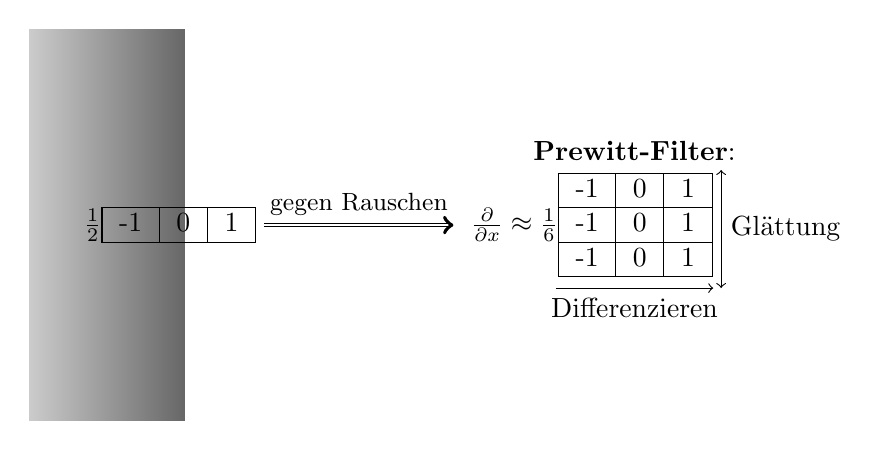
\begin{tikzpicture}
                    \draw[left color=black!20!white, right color=black!60,color=white] (0,0) rectangle (2,5);
                    \draw (1.8,2.5) node[] {$\frac{1}{2} \begin{tabular}{|c|c|c|}\hline
                        -1 & 0 & 1\\
                        \hline
                    \end{tabular}$};
                    \draw[->,double] (3,2.5) -- node[above] {\small gegen Rauschen}(5.4,2.5);
                    \draw (5.5,2.5) node[right] {$\frac{\partial }{\partial x} \approx  \frac{1}{6} \begin{tabular}{|c|c|c|}\hline
                        -1 & 0 & 1\\
                        \hline
                        -1 & 0 & 1\\
                        \hline
                        -1 & 0 & 1\\
                        \hline
                    \end{tabular}$};
                    \draw[->] (6.7,1.7) -- node[below] {Differenzieren} (8.7,1.7);
                    \draw[<->] (8.8,3.2) -- node[right] {Glättung} (8.8,1.7);
                    \draw (7.7,3.2) node[above] {\textbf{Prewitt-Filter}\index{Prewitt-Filter}:};
                \end{tikzpicture}
            \end{center}

            Alternative: $\frac{\partial }{\partial x} \approx \frac{1}{2} \begin{tabular}{|c|c|c|}\hline
                -1 & 0 & 1\\
                \hline
            \end{tabular} \boxast \frac{1}{4}\begin{tabular}{|c|c|c|}\hline
                1\\
                \hline
                2\\
                \hline
                1\\
                \hline
            \end{tabular} = \frac{1}{8} \begin{tabular}{|c|c|c|}\hline
            -1 & 0 & 1\\
            \hline
            -2 & 0 & 2\\
            \hline
            -1 & 0 & 1\\
            \hline
        \end{tabular}=:D_x$, genannt \textbf{Sobel-Filter}\index{Sobel-Filter}.
            Eine stärkere Glättung kann mittels anderer vertikaler Filter mit Binomialkoeffizienten erzielt werden.\\

            Entsprechen wird $\frac{\partial }{\partial y} D_y \coloneqq D_x^T$ definiert.\\

            \begin{equation}\label{eq:6.2}
                \nabla u(\x) = \srmatrix{\frac{\partial u}{\partial x}(\x)\\\frac{\partial u}{\partial y}(\x)} \approx \srmatrix{(D_x \boxast u)(\x)\\ (D_y \boxast u)(\x)}
            \end{equation}

            Zur Erinnerung der Gradienten steht senkrecht auf Kanten und zeigt in Richtung heller (hoher) Werte, die Intensität wird beschrieben von $\abs{\nabla u(\x)}$, also dem Betrag des Gradienten.

            Ein typischer Algorithmus kann etwa folgende Form annehmen:
            \begin{enumerate}
                \item Gradienten mittels Prewitt oder Sobel approximieren und Richtung auf Vielfache von $45^\circ$ runden.
                \item \textbf{Non-maximum suppression}\index{Non-maximum suppression} (edge thinning). Da es potentiell viele Punkte mit hoher Steigung gibt kann es dazu kommen, dass Kanten sehr breit werden, dieses wird durch das edge thinning verhindert.

            \begin{center}
                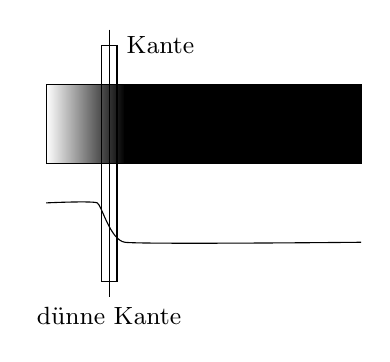
\begin{tikzpicture}
                    \draw[left color=white, right color=black] (0,0) rectangle (1,1);
                    \draw[fill] (1,0) rectangle (4,1);
                    \draw[shift={(0,-1)}] plot [smooth, tension = 0.2] coordinates {(0,0.5) (0.65,0.5) (1,0) (4,0)};
                    \draw (0.7,1.5) rectangle (0.9,-1.5);
                    \draw (0.9,1.5) node[right] {\small Kante};
                    \draw (0.8,1.7) -- (0.8,-1.7) node[below] {\small dünne Kante};
                \end{tikzpicture}
            \end{center}

            Mathematisch: $\x$ wird Kantenpunkt falls:
            \[\abs{\nabla u(\x)} \leq max(\abs{\nabla u(\x_+)},\abs{\nabla u(\x_-)})\]
            wobei $\x_+$ und $\x_-$ Vorgänger und Nachfolger von $\x$ in Gradientenrichtung sind.
            \item Kandidat $\x$ wird Kantenpunkt, falls:
            \begin{center}
                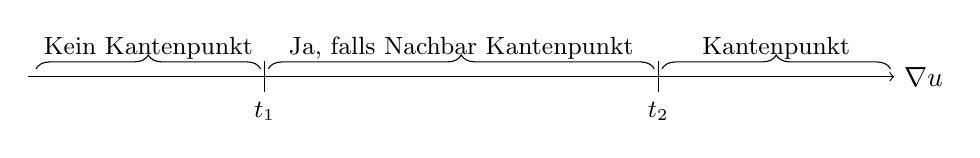
\begin{tikzpicture}
                    \draw[->] (0,0) -- (11,0) node[right] {$\abs{\nabla u}$};
                    \draw[decorate,decoration={brace,amplitude=5pt}] (0.1,0.1) -- node[above] {\small Kein Kantenpunkt} (2.95,0.1);
                    \draw[decorate,decoration={brace,amplitude=5pt}] (3.05,0.1) -- node[above] {\small Ja, falls Nachbar Kantenpunkt} (7.95,0.1);
                    \draw[decorate,decoration={brace,amplitude=5pt}] (8.05,0.1) -- node[above] {\small Kantenpunkt} (10.95,0.1);
                    \draw (3,0.2) -- (3,-0.2) node[below] {\small $t_1$};
                    \draw (8,0.2) -- (8,-0.2) node[below] {\small $t_2$};
                \end{tikzpicture}
            \end{center}
            wobei $t_1, \ t_2$ thresholds sind.\\
            $\x$ ist also ein Kantenpunkt, falls $\abs{\nabla u(\x)} \geq t_2$ oder $\left( \abs{\nabla u(\x)} \in [t_1,t_2] \text{ und $\x$ ist Nachbar eines Kantenpunktes}  \right)$.
            Dieses wird \textbf{hysteresis thresholding}\index{hysteresis thresholding} genannt und verhindert \textbf{Abreißen}\index{Abreißen} von Kantenzügen.
            \end{enumerate}

            Die am häufigsten verbreitete Version von 1) -3) ist der \textbf{Canny-Algorithmus}\index{Canny-Algorithmus} (1986).

            Matlab:
            \begin{lstlisting}
                BWimg=edge(u,'canny',[t_1, t_2],sigma);
            \end{lstlisting}

            \begin{enumerate}
                \item[BWimg:] Binärbild
                \item[u:] Graustufenbild
                \item[canny:]Algorithmus
                \item[$t_1, \ t_2$:] Sind gewählt wie oben
                \item[sigma:] Parameter für den Gaußkern aus 1)
            \end{enumerate}

        \subsection{Die zweite Ableitung}

            Zunächst in 1D:
            %Wenn jemand eine bessere Idee hat, kann er das gerne aufräumen.
            \begin{center}
                \begin{tikzpicture}
                    \draw[dotted] (-0.5,0) node[left] {\small $u$:}-- (8.5,0);
                    \draw[scale=1,domain=-2:0,smooth,variable=\x,shift ={(2,0)}] plot ({\x},{(e^((-(\x)^2)/(0.2))}) -- (4,1) [scale=1,domain=0:2,smooth,variable=\x,shift ={(4,0)}] plot({\x},{(e^((-(\x)^2)/(0.2))});

                    \draw[dotted] (-0.5,-2) node[left] {\small $u'$:}-- (8.5,-2);
                    \draw[scale=1,domain=-1.5:1,smooth,variable=\x,shift ={(1.5,-2)}] plot ({\x},{(e^((-(\x)^2)/(0.05))}) -- (4,0) [scale=1,domain=-1:1.5,smooth,variable=\x,shift ={(5,0)}] plot({\x},{-(e^((-(\x)^2)/(0.05))});

                    \draw[dotted] (-0.5,-4) node[left] {\small $u''$:}-- (8.5,-4);
                    \draw[scale=1,domain=-1.5:1,smooth,variable=\x,shift ={(1.5,-4)}] plot ({\x},{-5*\x*(e^((-(\x)^2)/(0.05))}) -- (4,0) [scale=1,domain=-1:1.5,smooth,variable=\x,shift ={(5,0)}] plot({\x},{5*\x*(e^((-(\x)^2)/(0.05))});

                    \draw(1.5,1.2)--(1.5,-4.5);
                    \draw(6.5,1.2)--(6.5,-4.5);
                    \draw[] (1.5,0.2865) node[circle,fill,inner sep=1pt] {};
                    \draw (6.5,0.2865) node[circle,fill,inner sep=1pt] {};
                    \draw (1.5,-1.02) node[circle,fill,inner sep=1pt] {};
                    \draw (6.5,-2.98) node[circle,fill,inner sep=1pt] {};
                    \draw (1.5,-4) node[circle,fill,inner sep=1pt] {};
                    \draw (6.5,-4) node[circle,fill,inner sep=1pt] {};
                \end{tikzpicture}
            \end{center}

            Test für Kantenpunkte $u''(\x) = 0$ und $\abs{u'(\x)}>$ threshold.\\
            Wichtig: Vorglätten!, da die 2. Ableitung noch anfälliger gegenüber Rauschen als die 1. Ableitung ist.\\
            \ \\
            In 2D. Laplace Operator $\Delta u = \frac{\partial^2 u}{\partial x^2} + \frac{\partial^2 u}{\partial y^2}$ (Richtungsunabhängige Messung der 2. Ableitung)\\
            Vorglätten: $\Delta (G * u) = (\Delta G)*u$, wobei $\Delta G$ vorher berechnet werden kann.

            In 1D:

            \begin{center}
                \begin{tikzpicture}
                    \draw (0,0.2) node[left] {$G:$};
                    \draw[scale=1,domain=-1.5:1.5,smooth,variable=\x,shift ={(2,0)}] plot ({\x},{(e^((-(\x)^2)/(0.2))});
                    \draw (4.5,0.2) node[left] {$\Delta G:$};
                    \draw[scale=0.5,domain=-4:4,smooth,variable=\x,shift ={(13,0)}] plot ({\x},{(\x*\x*(e^((-(\x)^2)/(2))) - (e^((-(\x)^2)/(2))});
                \end{tikzpicture}
            \end{center}

            In 2D:
            \def\centerx{2}
            \def\centery{-1}
            \begin{center}
                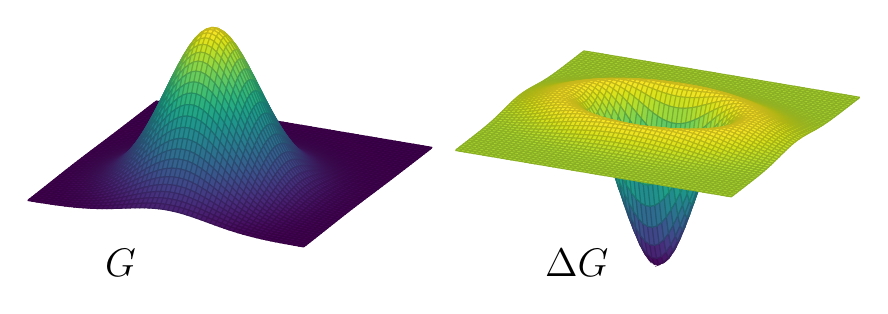
\begin{tikzpicture}
                \pgfplotsset{
                    colormap name=viridis,
                }
                    \begin{axis}[hide axis,scale=0.75,name=plot1]
                        \addplot3[surf,domain=-2:6,domain y=-3.7:3.7,samples=60]
                            {exp(-( (x-\centerx)^2 + (y-\centery)^2)/3 )};
                        \end{axis}
                        \draw[->] (6,1.5)--(7,1.5);
                        \draw (1.5,0) node[left] {\Large $G$};
                        \draw (7.5,0) node[left] {\Large $\Delta G$};
                    \begin{axis}[hide axis,scale=0.75,at={(8cm,1cm)}, anchor=center]
                        \addplot3[surf,domain=-3:3,domain y=-5:5,samples=60]
                        {x^2*exp(- x^2/2 - y^2/2) - 2*exp(- x^2/2 - y^2/2) + y^2*exp(- x^2/2 - y^2/2)};
                    \end{axis}
                \end{tikzpicture}
            \end{center}

            Dieses wird \textbf{Laplacian of Gaußian method}\index{Laplacian of Gaußian method} genannt.\\
            Matlab:
            \begin{lstlisting}
                BWimg=edge(u,'log',thresh,sigma);
            \end{lstlisting}
            $\Rightarrow$ alle $\x \in \Omega$ mit:
            \begin{enumerate}
                \item[] $\Delta (G_{sigma} * u)(\x) \approx u$, nicht auf Gleichheit sondern auf Vorzeichenwechsel testen.
                \item[und:] $\abs{\nabla(G_{sigma}) * u}>\text{thresh}$
            \end{enumerate}
